
\documentclass[12pt]{article}
\pagestyle{empty}
\setlength{\parskip}{0in}
\setlength{\textwidth}{6.8in}
\setlength{\topmargin}{-.5in}
\setlength{\textheight}{9.3in}
\setlength{\parindent}{0in}
\setlength{\oddsidemargin}{-.7cm}
\setlength{\evensidemargin}{-.7cm}

\usepackage{amsmath}
\usepackage{amsthm}
\usepackage{amstext}

\usepackage{graphicx}

\begin{document}


\textbf{MAT 105 Exam 1 (gray) Spring 2009} \hspace{.4in} {\large Name} \hrulefill

\begin{center}

\begin{tabular}
{|l|c|c|c|c|c|c|c|c|c|c|c|c|c|} \hline

 Problems & \hspace{5 pt} 1 \hspace{5 pt}  & \hspace{5 pt} 2 \hspace{5 pt} & \hspace{5 pt} 3 \hspace{5 pt} & \hspace{5 pt} 4 \hspace{5 pt} & \hspace{5 pt} 5 \hspace{5 pt} & \hspace{5 pt} Total  \hspace{5 pt} & &  \hspace{5 pt} Grade \hspace{5 pt}  \\ \hline
&&&&&&&&\\  
Points &&&&&&&    \hspace{.8in}\% &  \\ 
&&&&&&&& \\  \hline
Out of & 12 & 32 & 32 & 14 & 10 &100 & & \\ \hline

\end {tabular}

\end{center}

\vspace{.2in}

 \emph{Relax.  You have done problems like these before.  Even if these problems look a bit different, just do what you can.  If you're not sure of something, please ask! You may use your calculator.  Please show all of your work and write down as many steps as you can.  Don't spend too much time on any one problem.  Always remember to report the units on an answer. Do well.  And remember, ask me if you're not sure about something.}\\

\vspace{.5in} 
\noindent \emph{A few formulas from our book:}

\begin{center}

\textbf{Root Formula:} 

A solution of the equation $B^n=k$ is $B=k^{1/n}$.

\vspace{.2in} 

\textbf{Percent Increase Formula:} 

To get the result of increasing an amount by $r$\%, multiply by $1 + \frac{r}{100}$.

\end{center}

\hrulefill

%%%%%%%%%%%

\newpage

\begin{enumerate}
%%% Old 1.3, air quality, citizen
\item Khalid is concerned about the environment and hence is investigating the emissions of a local garbage incinerator.  The graph below shows the amount of sulfur dioxide ($S$, units of grams per cubic meter) in the air a distance $D$ (in miles) from the plant. Large amounts of sulfur dioxide in the air cause a phenomena known as acid rain. Use the graph to answer the following questions.

\begin{center}
\scalebox {.7} {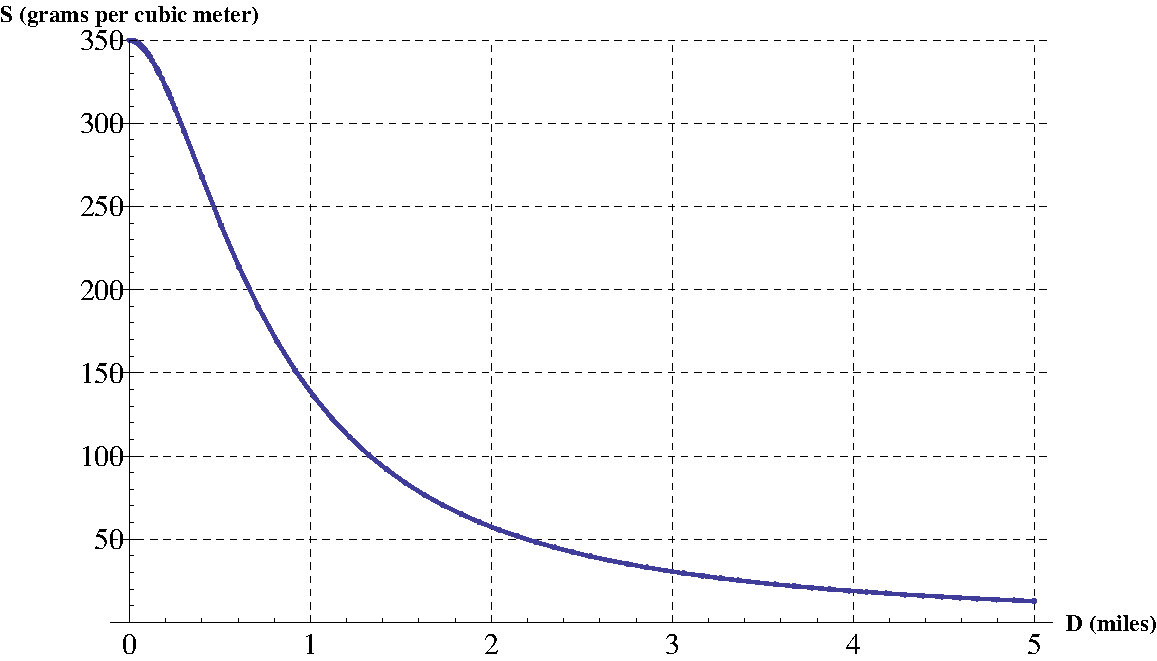
\includegraphics [width = 8in] {garbageEmissions_B}}
\end{center}



\begin{enumerate}
\item How much sulfur dioxide is in the air at the incinerator?
\vfill
\item What is the sulfur dioxide concentration 1 mile from the incinerator?
\vfill
\item How far away from the incinerator is the sulfur dioxide concentration at 100 grams per cubic meter?
\vfill
\item About how far away from the plant is the sulfur dioxide concentration below 50 grams per cubic meter?
\vfill
\end{enumerate}

%%%%%%%%%%%%%%%%%%%%%%%%%
\newpage
%%% Old 1.6, home, everyday
\item  To purchase stamps at my ATM there is a \$0.75 convenience fee.  Each stamp costs 42 cents.   

\begin{enumerate}
\item Make a table showing the cost to buy 5 stamps, 10 stamps, and 20 stamps from the ATM.
\vfill
\item Name the variables, including units, and write an equation illustrating the dependence.
\vfill
\item My wife bought stamps from the ATM and it cost her \$13.35.  Solve your equation to determine how many stamps she bought.  \emph{If you cannot solve the equation, you may show some other method of finding the answer for possible partial credit.}
\vfill
\item Draw a graph showing how the cost of buying stamps changes with the number of stamps purchased.
\vspace{.1in}
\begin{center}
\scalebox {.8} {
\includegraphics [width = 6in] {../GraphPaper}}
\end{center}
\vspace{.1in}
\end{enumerate}

%%%%%%%%%%%%%%%%%%%%%%%%%%%%%%%%%%%
\newpage

%%% Old 1.8, population, citizen?
\item The CIA world factbook estimated that the population of Costa Rica is growing at a rate of 1.3\% per year.  In 2008 the population was estimated to be 4.2 million.  

\begin{enumerate}
\item Write an equation illustrating this dependence using the following variables:

\quad $P= $ population (measured in millions of people)

\quad $Y = $ year (measured in years since 2008)

\vfill
\item Make a table showing the population in 2008, 2013, 2018, and 2023. Please report your answer to the first decimal place.
\vfill
\item Draw a graph showing how population will change in the future.
\vspace{.1in}
\begin{center}
\scalebox {.8} {
\includegraphics [width = 6in] {../GraphPaper}}
\end{center}
\vspace{.1in}
\item Use successive approximations to predict when the population will rise above 5 million.  Please report your answer to the first decimal place.   \emph{Display your work in a table.  Answer to the nearest year.  Be sure to say the actual year.}
\vfill
\vfill
\end{enumerate}


%%%%%%%%%%%%%%%%%
\newpage
%%% Old 1.7, physics, everyday
\item When you apply the brakes to stop a bicycle, you don't actually stop immediately.  The distance it takes depends on how fast you were going.  For one bike tested, $D = 0.23 S^2$, where $S$ is the speed of the bike (in mph) and $D$ is the distance before stopping (in feet).

\begin{enumerate}
\item Make a table showing the shopping distances for speeds of 5, 10, 15, and 20 mph.  Please report your answer to the first decimal place.
\vfill
\item Approximately how fast can a bike go and still be able to stop within 30 feet?  Please report your answer to the first decimal place.

\emph{You may use whatever method you prefer to answer the question, but please give an answer accurate to one decimal place.}
\vfill

\end{enumerate}

\noindent \hrulefill
%%% Old 1.4, gas prices, fun
\item In Saudi Arabia, gasoline prices are recorded in riyals/liter.  (The riyal is the currency of Saudi Arabia).  The average price of gasoline in Saudi Arabia is 0.45 riyals/liter.  What would that price be in terms of US dollars per gallon?

\emph{Useful facts:  \$1.00 $\approx$ 3.70 riyals and 1 gallon $\approx$ 3.8 liters }
\vfill


\end{enumerate}



%%%%%%%%%%%%%%%%

\newpage




\end{document}
